\documentclass[a4paper,11pt]{article}
\usepackage[latin1]{inputenc}
\usepackage[T1]{fontenc}
\usepackage{bbm}
\usepackage{amsmath}
\usepackage{indentfirst}
\usepackage{fullpage}
\usepackage{url}
\usepackage{geometry}
\geometry{verbose,tmargin=3cm,bmargin=2cm,lmargin=2cm,rmargin=2cm}
\usepackage{graphicx}
\usepackage{epstopdf}
\usepackage[center,footnotesize]{caption}
\usepackage[section]{placeins}
\usepackage{subfig}
\DeclareRobustCommand{\greektext}{%
  \fontencoding{LGR}\selectfont\def\encodingdefault{LGR}}
\DeclareRobustCommand{\textgreek}[1]{\leavevmode{\greektext #1}}
\DeclareFontEncoding{LGR}{}{}
\DeclareTextSymbol{\~}{LGR}{126}
\title{Series 4}
\date{October 11, 2011}
\author{Genomics and bioinformatics - Week 4}
\begin{document}
\maketitle




\section{Sequence alignment}
The Needlman-Wunsch algorithm uses a method called ``dynamic programming''. This is a very general programming technique. It involves three main steps:
\begin{enumerate}
\item Initialization
\item Scoring (matrix fill)
\item Alignment (backtracking)
\end{enumerate}
In the first exercise of this session you will manually perform a global alignment of two sequences based on the following scoring scheme:
\emph{Match:} \texttt{+1}, \emph{Mismatch:} \texttt{-1}, \emph{Gap:} \texttt{-2}\\
Sequence 1: \texttt{GAATTCAG}\\
Sequence 2: \texttt{GGATCG}.
\vspace{0.5cm}
\begin{center}

\includegraphics[width=0.8\textwidth]{matrix.png}
\end{center}
\vspace{0.5cm}

The best alignment is: ........\\

 
\section{Pair Hidden Markov Model}

In this exercise, we will construct a pair Hidden Markov Model for
the same sequences as in the first exercise and align them using the
path with maximum probability. The maximum probability of generating
the alignment and the corresponding path are calculated by a dynamic
programming algorithm which is called the Viterbi Algorithm. You will
see through the exercise that the Viterbi algorithm is actually similar
to the Needleman-Wunsch algorithm.

%
\begin{figure}[h]
\begin{center}
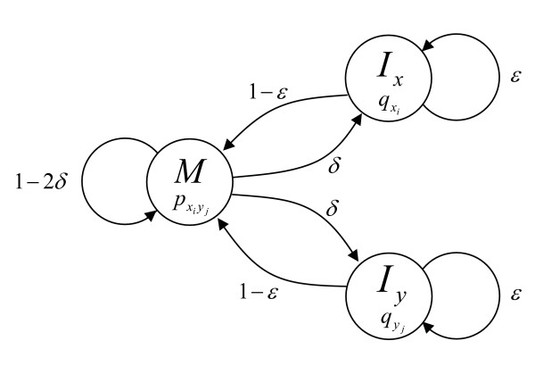
\includegraphics[width=0.5\textwidth]{HMM.jpg}\caption{Pair Hidden Markov Model}

\end{center}

%
\end{figure}


The Pair HMM consists of the following parameters(Figure)

\vspace{0.5cm}

Three states: M, I, D

State M matches one letter from each sequence

State I (Insertion) inserts a gap to the second sequence

State D (Deletion) inserts a gap to the first sequence\\


So, three states will be denoted by M, I and D in the algorithm written below.
\vspace{0.5cm}

Emission probabilities: p(x, y), q(x) and q(y), where

p(x,y) = probability of emitting a pair of characters {[}x,y{]}

q(x) = probability of emitting a pair of character {[}x,\_{]}

q(y) = probability of emitting a pair of character {[}\_,y{]}

\vspace{0.5cm}

Transition probabilities:

\textgreek{d} = probability of opening a gap

\textgreek{e} = probability of extending a gap

\vspace{0.5cm}
The algorithm goes through the three steps:\\


Step 1: Initialization
\[
VM(0,0)=0; VD(0,0)=-\infty ; VI(0,0)=-\infty;
V*(-1,j)=V*(i,-1)=-\infty;\]
\newpage


Step 2: Recursion

\[ VM(i,j) =S(x_{i},y_{j})+max \left\{ \begin{array}{ll}
	 VM(i-1,j-1)\\
         VD(i-1,j-1) \\
         VI(i-1,j-1)  .\end{array} \right. \] 

\[ VD(i,j) =max \left\{ \begin{array}{ll}
         VM(i-1,j)-d \\
         VD(i-1,j)-e  .\end{array} \right. \] 

\[ VI(i,j) =max \left\{ \begin{array}{ll}
         VM(i,j-1)-d \\
         VI(i,j-1)-e  .\end{array} \right. \]  



Step 3: Termination

\[ VE=max(VM(n,m),VD(n,m),VI(n,m))\]\\

To make correspondence to the Needleman-Wunsch algorithm with the scores given in Exercise 1,

\[
S(x,y)=log\frac{p(x,y)}{p(x)\; p(y)}\]

\[
d=-log(\delta)\]

where 

S(x,y) = 1 for match, 

S(x,y) = -1 for mismatch,

d = -2 for gap penalty.

\begin{enumerate}
\item Deduce the emission probability matrix and the transition probabilities for the HMM
\item Use the algorithm as shown above to generate the three matrices for Match(M), Delete(D) and Insertion(I)
\item Deduce the alignment based on the three matrices.
\end{enumerate}

\underline{Solution:}
\newpage

Matrix $V_M$:
\begin{center}

\includegraphics[width=0.8\textwidth]{matrix.png}
\end{center}
\vspace{1.5cm}

Matrix $V_D$:
\begin{center}

\includegraphics[width=0.8\textwidth]{matrix.png}
\end{center}
\vspace{1.5cm}

\newpage 

Matrix $V_I$: 
\begin{center}

\includegraphics[width=0.8\textwidth]{matrix.png}
\end{center}
\vspace{0.5cm}

Backtracking matrix:
\begin{center}

\includegraphics[width=0.8\textwidth]{matrix.png}
\end{center}
\vspace{0.5cm}

The possible alignments are: ........................


\end{document}
